\ProvidesPackage{commands}
\documentclass[11pt]{article}
\usepackage{epstopdf}
\usepackage{subfigure,graphicx}
\usepackage{amsmath}
\usepackage{epsf}
\usepackage{amsfonts}
\usepackage{amssymb}
\usepackage{color}
\usepackage{mathtools}
\usepackage{placeins}
\usepackage{booktabs}
\usepackage{enumitem}
\usepackage{caption}
\usepackage[margin=0.8in, paperwidth=8.5in, paperheight=11in]{geometry}
\usepackage{amsfonts}
\usepackage{amsmath}
\usepackage{amsbsy}
\usepackage{authblk}
\usepackage{graphicx}
\usepackage{listings}
\usepackage{array}
\usepackage{titlesec}
\usepackage{amssymb}
\usepackage{bm}
\usepackage{mathtools}
\usepackage{titlesec}

\usepackage[latin1]{inputenc}\newcommand{\bs}[1]{\boldsymbol{#1}}
\newcommand{\del}[2]{\frac{\partial {#1}}{\partial {#2}}}
\newcommand{\D}[2]{\frac{D^{\overline{\alpha}}}{\overline{\alpha !}}{#1}(#2,#2)\ {\bf x}^{\overline{\alpha}}}
\newcommand{\dv}[3]{\frac{{\rm d}^{#1}{#2}}{d{#3}^{#1}}}
\newcommand{\ddel}[5]{\frac{\partial^{ {#1} + {#2}} {#3}}{\partial {#4}^{#1} \partial{#5}^{#2}}}
\newcommand{\dev}{{\rm {\bf dev}}}
\newcommand{\proj}[1]{\frac{1}{R^2}{\bf X}\otimes{\bf X}}
\newcommand{\Ie}[1]{I^{\rm e}_{#1}}
\newcommand{\Ce}[1]{\bf C^{\rm e^{#1}}}
\newcommand{\Fe}[2]{F^{\rm e^{#2}}_{#1}}
\newcommand{\Fv}[2]{F^{\rm v^{#2}}_{#1}}
\newcommand{\f}[2]{f^{\rm {#2}}_{#1}}
\newcommand{\B}[2]{B^{\rm {#2}}_{#1}}
\newcommand{\E}[2]{E^{\rm {#2}}_{#1}}
\newcommand{\fv}[2]{f^{\rm v^{#2}}_{#1}}
\newcommand{\dfv}[2]{\dot{f}^{\rm v^{#2}}_{#1}}
\newcommand{\tGam}[2]{\tilde{\Gamma}^{\rm v^{#2}}_{#1}}
\newcommand{\Gam}[2]{\Gamma^{\rm v^{#2}}_{#1}}
\newcommand{\A}[1]{\mathcal{A}_{#1}}
\newcommand{\F}[2]{F^{\rm #2}_{#1}}
\newcommand{\hpeq}{\hat{\psi}^{\rm Eq}}
\newcommand{\hpneq}{\hat{\psi}^{\rm NEq}}
\newcommand{\etak}{\eta_K({I_1,I_2,J},{\bf C^{\rm e}, B^{\rm v}})}
\newcommand{\nuk}{\nu_K({I_1,I_2,J},{\bf C^{\rm e}, B^{\rm v}})}
\newcommand{\thetak}{\theta_K({I_1,I_2,J},{\bf C^{\rm e}, B^{\rm v}})}
\newcommand{\etaj}{\eta_J({I_1,I_2,J},{\bf C^{\rm e}, B^{\rm v}})}
\newcommand{\dFv}[2]{\dot{F}^{\rm v^{#2}}_{#1}}
\newcommand{\hatpsi}{\widehat{\psi}(I_1, I_2,I^{\rm e}_1,I^{\rm e}_2,J)}
\newcommand{\hpsi}{\widehat{\psi}(I_1,I^{\rm e}_1,J)}
\newcommand{\Fh}[1]{\widehat{\mathcal{F}}\left({\bf F, \Fv{}{}}, {#1}\right)}
\newcommand{\Fhstar}[1]{\widehat{\mathcal{F}}^*\left({\bf F, \Fv{}{}}, {#1}\right)}
\newcommand{\sbar}{\overline{\bm{\sigma}}}
\newcommand{\hpsicomp}[1]{\sum_{r=1}^{2}\left\{\frac{3^{1-\alpha_r}}{2\alpha_r}\mu_r(I^{\alpha_r}_1-3^{\alpha_r})
+\frac{3^{1-a_r}}{2a_r}m_r({\Ie{1}}^{^{a_r}}-3^{a_r})\right\}
+\mu{#1}+\kappa{#1}^2}
\newcommand{\Ni}[1]{N^{(e)}_i(#1)}
\newcommand{\hNi}[1]{\hat{{N}}^{(e)}_i(#1)}
\newcommand{\Ld}{L^{\dagger}}
\newcommand{\intinfinf}{\int_{-\infty}^{\infty} \int_{-\infty}^{\infty}}
\newcommand{\LLnorm}[1]{\left\lVert{#1}\right\rVert_2}
\newcommand{\Linorm}[1]{{\left\lVert{#1}\right\rVert_\infty}}
\newcommand{\tr}{\rm tr}
\newcommand{\deldel}[2]{\frac{\partial^2 {#1}}{\partial {#2}^2}}
\newcommand{\kd}[1]{\delta_{#1}}
\newcommand{\Fie}[1]{{\bf F}^{#1}}
\newcommand{\Comp}{\emph{CompStrainStress\_Cee570.m}}
\newcommand{\Comps}{\emph{CompStrainStress\_Elem\_Cee570.m}}
\newcommand{\Feap}{\emph{FEA\_Program.m}}
\newcommand{\Elast}{\emph{Elast2d\_Elem.m}}
\newcommand{\Assem}{\em{AssemStifForc.m}}
\newcommand{\Fb}{\em{F\_bar\_int}}
\newcommand{\Form}{\em{FormFE.m}}
\newcommand{\Sol}{\em{SolveFE.m}}
\newcommand{\inpt}{\em{triangtwo.m}}

\titlespacing\section{10pt}{10pt plus 4pt minus 2pt}{10pt plus 2pt minus 2pt}
\titlespacing\subsection{0pt}{8pt plus 4pt minus 2pt}{8pt plus 2pt minus 2pt}
\titlespacing\subsubsection{0pt}{12pt plus 4pt minus 2pt}{6pt plus 2pt minus 2pt}
\titlespacing*{\title}{-2ex}{*-2ex}{-2ex}
\usepackage{color} %red, green, blue, yellow, cyan, magenta, black, white
\definecolor{mygreen}{RGB}{28,172,0} % color values Red, Green, Blue
\definecolor{mylilas}{RGB}{170,55,241}
\setlength\parindent{0pt}
\graphicspath{{Figures/}}

\usepackage{graphicx}
\title{\bf CEE 576: Nonlinear Finite Elements \\ HW6}
\author{Bhavesh Shrimali \\ NetID: bshrima2}
\date{\today}
\begin{document}
\maketitle \hrule
\section*{Problem 1: }
From class lectures, we have the element level matrix-system as follows: 
\begin{align*}
\begin{bmatrix}[1.5]
\frac{E}{h} & 0 & -\frac{E}{h} & 0\\
-\frac{m}{2\Delta t} & \frac{\overline{c}h}{2\Delta t}+ \frac{\overline{k}}{2h} & \frac{m}{2\Delta t} & -\frac{\overline{k}}{2h} \\
-\frac{E}{h} & 0 & \frac{E}{h} & 0 \\
- \frac{m}{2\Delta t} & - \frac{\overline{k}}{2h} & \frac{m}{2\Delta t} & \frac{\overline{c}h}{2\Delta t}+ \frac{\overline{k}}{2h}
\end{bmatrix}
\begin{Bmatrix}[1.5]
d^e_1\\d^e_2\\d^e_3\\d^e_4
\end{Bmatrix}_{n+1}
= 
\begin{bmatrix}[1.5]
0 & -\frac{m}{2} & 0 & -\frac{m}{2}\\
-\frac{m}{2\Delta t} & \frac{\overline{c}h}{2\Delta t}-\frac{\overline{k}}{2h} & \frac{m}{2\Delta t} & \frac{\overline{k}}{2h} \\
0 & \frac{m}{2} & 0 & \frac{m}{2}\\
- \frac{m}{2\Delta t} & \frac{\overline{k}}{2h} &  \frac{m}{2\Delta t} & \frac{\overline{c}h}{2\Delta t}- \frac{\overline{k}}{2h}
\end{bmatrix} 
\begin{Bmatrix}[1.5]
d^e_1\\d^e_2\\d^e_3\\d^e_4
\end{Bmatrix}_{n}
\end{align*}\hrule
\subsection*{(a): }
For the present problem: 
\begin{itemize}
\item $d^e_1$ and $d^e_2$ correspond to the axial displacement and temperature at the left end, i.e. node 1 and $d^e_3$ and $d^e_4$ correspond to the axial displacement and temperature at the right end, i.e. node 2. 
\item We are given that the displacement and temperature at the right node are specified to be zero. And hence we would get a 2x2 linear system for our element, given as below:
\end{itemize}
\begin{align*}
\begin{bmatrix}[1.5]
\frac{E}{h} & 0 \\
-\frac{m}{2\Delta t} & \frac{\overline{c}h}{2\Delta t}+ \frac{\overline{k}}{2h}
\end{bmatrix}
\begin{Bmatrix}[1.5]
d^e_1 \\ d^e_2
\end{Bmatrix}_{n+1}
=
\begin{bmatrix}[1.5]
0 & -\frac{m}{2} \\
-\frac{m}{2\Delta t} & \frac{\overline{c}h}{2\Delta t}-\frac{\overline{k}}{2h} 
\end{bmatrix}
\begin{Bmatrix}[1.5]
d^e_1 \\ d^e_2
\end{Bmatrix}_{n}
\end{align*}
For the next part it is worthwhile to note that the assembly process can be done efficiently using block matrices. While directly adding the block matrices, for each of the elements, the only entries that are affected are $(3,3),(3,4),(4,3),(4,4)$ and so on as follows: 
\begin{itemize}
\item The entry in $(3,3)$ gets added to the entry in $(1,1)$ for the next element
\item The entry in $(3,4)$ gets added to the entry in $(1,2)$ for the next element
\item The entry in $(4,3)$ gets added to the entry in $(2,1)$ for the next element
\item The entry in $(4,4)$ gets added to the entry in $(2,2)$ for the next element
\end{itemize} 
Thus the system stiffness matrix can be readily assembled as given below
\subsection*{(b): }
We assume equal mesh size for each element and therefore readily assemble the block matrices as explained above: 
\begin{align*}
{\bf A}_{n+1}
& =
\begin{bmatrix}[1.5]
\frac{E}{h} & 0 & -\frac{E}{h} & 0 & 0 & 0 & 0 & 0\\
-\frac{m}{2\Delta t} & \frac{\overline{c}h}{2\Delta t}+ \frac{\overline{k}}{2h} & \frac{m}{2\Delta t} & -\frac{\overline{k}}{2h} & 0 & 0 & 0 & 0 \\
-\frac{E}{h} & 0 & \frac{2E}{h} & 0 & -\frac{E}{h} & 0 & 0 & 0 \\
- \frac{m}{2\Delta t} & - \frac{\overline{k}}{2h} & 0 & \frac{\overline{c}h}{\Delta t} + \frac{\overline{k}}{h} & \frac{m}{2\Delta t} & -\frac{\overline{k}}{2h} & 0 & 0 \\
0 & 0 & -\frac{E}{h} & 0 & \frac{2E}{h} & 0 & -\frac{E}{h} & 0 \\
0 & 0 & -\frac{m}{2\Delta t} & -\frac{\overline{k}}{2h} & 0 & \frac{\overline{c}h}{\Delta t} + \frac{\overline{k}}{h} & \frac{m}{2\Delta t} & -\frac{k}{2h} \\
0 & 0 & 0 & 0 & -\frac{E}{h} & 0 & \frac{2E}{h} & 0 \\
0 & 0 & 0 & 0 & -\frac{m}{2\Delta t} & -\frac{\overline{k}}{2h} & 0 & \frac{\overline{c}h}{\Delta t} + \frac{\overline{k}}{h}
\end{bmatrix} \\ \\
{\bf A}_n
& =
\begin{bmatrix}[1.5]
0 & -\frac{m}{2} & 0 & -\frac{m}{2} & 0 & 0 & 0 & 0\\
-\frac{m}{2\Delta t} & \frac{\overline{c}h}{2\Delta t}-\frac{\overline{k}}{2h} & \frac{m}{2\Delta t} & \frac{\overline{k}}{2h}  & 0 & 0 & 0 & 0\\
0 & \frac{m}{2} & 0 & 0 & 0 & -\frac{m}{2} & 0 & 0\\
- \frac{m}{2\Delta t} & \frac{\overline{k}}{2h} &  0 & \frac{\overline{c}h}{\Delta t}- \frac{\overline{k}}{h} & \frac{m}{2\Delta t} & \frac{\overline{k}}{2h}  & 0 & 0\\
0 & 0 & 0 & \frac{m}{2} & 0 & 0 & 0 & -\frac{m}{2}\\
0 & 0 & -\frac{m}{2\Delta t} & \frac{\overline{k}}{2h} & 0 & \frac{\overline{c}h}{\Delta t}- \frac{\overline{k}}{h} & \frac{m}{2\Delta t} & \frac{\overline{k}}{2h} \\
0 & 0 & 0 & 0 & 0 & \frac{m}{2} & 0 & 0 \\
0 & 0 & 0 & 0 & -\frac{m}{2\Delta t } & \frac{\overline{k}}{2h} & 0 & \frac{\overline{c}h}{\Delta t}- \frac{\overline{k}}{h}
\end{bmatrix}
\end{align*}
and the corresponding linear system is given by 
\begin{align*}
{\bf A}_{n+1}{\bf d}_{n+1}
=
{\bf A}_{n}{\bf d}_n
\end{align*}
where 
\begin{align*}
{\bf d}_{n+1}
=
\begin{Bmatrix}[1.5]
d^e_1\\d^e_2\\d^e_3\\d^e_4\\d^e_5\\d^e_6\\d^e_7\\d^e_8
\end{Bmatrix}_{n+1} \ \ \text{and} \ \ \ \ \ 
{\bf d}_{n}
=
\begin{Bmatrix}[1.5]
d^e_1\\d^e_2\\d^e_3\\d^e_4\\d^e_5\\d^e_6\\d^e_7\\d^e_8
\end{Bmatrix}_{n}
\end{align*}\hrule\newpage
\subsection*{(c): Numerical Implementation}
The numerical implementation of the Isothermal split is as follows:
\begin{itemize}
\item E = 100
\item m = 0.3 
\item $\overline{k}$ = 1.0
\item $\overline{c}$ = 1.0
\item L = 1.0
\item h = 0.25
\end{itemize}
\subsubsection*{(ii):}
The element level stiffness matrix-system for a two noded 1-D linear element (upon substitution of the above material parameters), for $\Delta t = 0.05s$, can be obtained as 
\begin{align*}
{\bf A}_{n+1}
{\bf d}^e_{n+1}
=
{\bf A}_{n}
{\bf d}^e_{n} \implies {\bf d}^e_{n+1} = {{\bf A}_{n+1}}^{-1}
\left( 
{\bf A}_{n}
{\bf d}^e_{n}
\right)
\end{align*}
where the matrices are as defined in the previous part
The corresponding values are tabulated as follows: \\
\begin{table}[htbp]
  \centering
  \caption{Isothermal Split: Evolution of Displacement ({\bf D}) and Temperature ({\bf T}) ($\Delta t = 0.05$)}
    \begin{tabular}{rcrrrrrrr}
    \toprule
    \multicolumn{1}{l}{\textbf{Node}} & \multicolumn{1}{l}{\textbf{Quantity}} & \multicolumn{1}{l}{\textbf{n = 1}} & \multicolumn{1}{l}{\textbf{n = 2}} & \multicolumn{1}{l}{\textbf{n = 3}} & \multicolumn{1}{l}{\textbf{n = 4}} & \multicolumn{1}{l}{\textbf{n = 5}} & \multicolumn{1}{l}{\textbf{n = 6}} & \multicolumn{1}{l}{\textbf{n = 7}} \\
    \midrule
    \multicolumn{1}{l}{\textbf{Node 1}} & \textbf{D} & 0.1   & -0.00066 & -0.00051 & -0.00045 & -0.0004 & -0.00035 & -0.00031 \\
          & \textbf{T} & 0.25  & 0.24585 & 0.231223 & 0.208083 & 0.18473 & 0.163897 & 0.145178 \\
    \multicolumn{1}{l}{\textbf{Node 2}} & \textbf{D} & 0.1   & -0.00047 & -0.00032 & -0.00028 & -0.00025 & -0.00022 & -0.00019 \\
          & \textbf{T} & 0.25  & 0.240945 & 0.217837 & 0.192523 & 0.171071 & 0.151489 & 0.134165 \\
    \multicolumn{1}{l}{\textbf{Node 3}} & \textbf{D} & 0.1   & -0.00028 & -0.00015 & -0.00014 & -0.00012 & -1.03E-04 & -9.08E-05 \\
          & \textbf{T} & 0.25  & 0.213964 & 0.168725 & 0.149343 & 0.13135 & 0.11614 & 0.102741 \\
    \multicolumn{1}{l}{\textbf{Node 4}} & \textbf{D} & 1.00E-01 & -9.38E-05 & -3.65E-05 & -3.60E-05 & -3.05E-05 & -2.68E-05 & -2.36E-05 \\
          & \textbf{T} & 0.25  & 0.097454 & 0.095913 & 0.081345 & 0.071421 & 0.062938 & 0.055637 \\
    \midrule
    \multicolumn{1}{l}{\textbf{Node}} & \multicolumn{1}{l}{\textbf{Quantity}} & \multicolumn{1}{l}{\textbf{n = 8}} & \multicolumn{1}{l}{\textbf{n = 9}} & \multicolumn{1}{l}{\textbf{n = 10}} & \multicolumn{1}{l}{\textbf{n = 11}} &       &       &  \\
\cmidrule{1-6}    \multicolumn{1}{l}{\textbf{Node 1}} & \textbf{D} & -0.00027 & -0.00024 & -0.00021 & -0.00019 &       &       &  \\
          & \textbf{T} & 0.128563 & 0.113827 & 0.100776 & 0.089218 &       &       &  \\
    \multicolumn{1}{l}{\textbf{Node 2}} & \textbf{D} & -0.00017 & -0.00015 & -0.00013 & -0.00012 &       &       &  \\
          & \textbf{T} & 0.118786 & 0.105167 & 0.093106 & 0.082427 &       &       &  \\
    \multicolumn{1}{l}{\textbf{Node 3}} & \textbf{D} & -8.03E-05 & -7.10E-05 & -6.29E-05 & -5.56E-05 &       &       &  \\
          & \textbf{T} & 0.090936 & 0.080498 & 0.071262 & 0.063088 &       &       &  \\
    \multicolumn{1}{l}{\textbf{Node 4}} & \textbf{D} & -2.09E-05 & -1.85E-05 & -1.63E-05 & -1.45E-05 &       &       &  \\
          & \textbf{T} & 0.049225 & 0.043569 & 0.038568 & 0.034143 &       &       &  \\
\cmidrule{1-6}    \end{tabular}%
  \label{tab:addlabel}%
\end{table}%

\subsubsection*{(iii):}
The element level stiffness matrix-system for a two noded 1-D linear element (upon substitution of the above material parameters), for $\Delta t = 0.1s$, can be obtained as 
\begin{align*}
{\bf A}_{n+1}
{\bf d}^e_{n+1}
=
{\bf A}_{n}
{\bf d}^e_{n} \implies {\bf d}^e_{n+1} = {{\bf A}_{n+1}}^{-1}
\left( 
{\bf A}_{n}
{\bf d}^e_{n}
\right)
\end{align*}
The corresponding values are tabulated below: 
\begin{table}[htbp]
  \centering
  \caption{Isothermal Split: Evolution of Displacement ({\bf D}) and Temperature ({\bf T}) ($\Delta t = 0.1s$)}
    \begin{tabular}{rcrrrrrr}
    \toprule
    \multicolumn{1}{l}{\textbf{Node }} & \multicolumn{1}{l}{\textbf{Quantity}} & \multicolumn{1}{l}{\textbf{n =1 }} & \multicolumn{1}{l}{\textbf{n = 2 }} & \multicolumn{1}{l}{\textbf{n = 3}} & \multicolumn{1}{l}{\textbf{n = 4}} & \multicolumn{1}{l}{\textbf{n = 5}} & \multicolumn{1}{l}{\textbf{n = 6}} \\
    \midrule
    \multicolumn{1}{l}{\textbf{Node 1}} & \textbf{D} & 0.1   & -0.00066 & -0.00043 & -0.00035 & -0.00027 & -0.00021 \\
          & \textbf{T} & 0.25  & 0.233658 & 0.189026 & 0.143323 & 0.113196 & 0.088681 \\
    \multicolumn{1}{l}{\textbf{Node 2}} & \textbf{D} & 0.1   & -0.00047 & -0.00026 & -0.00022 & -0.00017 & -0.00013 \\
          & \textbf{T} & 0.25  & 0.223585 & 0.171192 & 0.132565 & 0.1051 & 0.081438 \\
    \multicolumn{1}{l}{\textbf{Node 3}} & \textbf{D} & 0.1   & -0.00028 & -0.00011 & -1.06E-04 & -7.82E-05 & -6.30E-05 \\
          & \textbf{T} & 0.25  & 0.180774 & 0.120565 & 0.106258 & 0.078183 & 0.063409 \\
    \multicolumn{1}{l}{\textbf{Node 4}} & \textbf{D} & 1.00E-01 & -9.38E-05 & -1.94E-05 & -3.03E-05 & -1.92E-05 & -1.69E-05 \\
          & \textbf{T} & 0.25  & 0.051712 & 0.080827 & 0.05114 & 0.044956 & 0.033196 \\
    \bottomrule
    \end{tabular}%
  \label{tab:addlabel}%
\end{table}\hrule
\section*{Problem 2: }
For the present problem: 
\begin{itemize}
\item $d^e_1$ and $d^e_2$ correspond to the axial displacement and temperature at the left end, i.e. node 1 and $d^e_3$ and $d^e_4$ correspond to the axial displacement and temperature at the right end, i.e. node 2. 
\item We are given that the displacement and temperature at the right node are specified to be zero. And hence we would get a 2x2 linear system for our element, given as below:
\end{itemize}
For the Adiabatic split, we have the element level matrix-system as follows: 
\begin{align*}
\begin{bmatrix}[1.5]
\frac{E}{h} & \frac{m}{4} & -\frac{E}{h} & \frac{m}{4}\\
-\frac{m}{2\Delta t} & \frac{\overline{c}h}{2\Delta t}+ \frac{\overline{k}}{h} & \frac{m}{2\Delta t} & -\frac{\overline{k}}{h} \\
-\frac{E}{h} & -\frac{m}{4} & \frac{E}{h} & -\frac{m}{4} \\
- \frac{m}{2\Delta t} & - \frac{\overline{k}}{h} & \frac{m}{2\Delta t} & \frac{\overline{c}h}{2\Delta t}+ \frac{\overline{k}}{h}
\end{bmatrix}
\begin{Bmatrix}[1.5]
d^e_1\\d^e_2\\d^e_3\\d^e_4
\end{Bmatrix}_{n+1}
= 
\begin{bmatrix}[1.5]
0 & -\frac{m}{4} & 0 & -\frac{m}{4}\\
-\frac{m}{2\Delta t} & \frac{\overline{c}h}{2\Delta t} & \frac{m}{2\Delta t} & 0 \\
0 & \frac{m}{4} & 0 & \frac{m}{4}\\
- \frac{m}{2\Delta t} & 0 &  \frac{m}{2\Delta t} & \frac{\overline{c}h}{2\Delta t}
\end{bmatrix} 
\begin{Bmatrix}[1.5]
d^e_1\\d^e_2\\d^e_3\\d^e_4
\end{Bmatrix}_{n}
\end{align*}
\subsection*{(a): }
The one-element mesh has zero Dirichlet conditions at the right node, i.e., $d^e_3 = d^e_4 = 0$ at $t=t_n$ and $t=t_{n+1}$, and hence the element level matrix-system would comprise of only the first two rows and first two columns of the above system: 
\begin{align*}
\begin{bmatrix}[1.5]
\frac{E}{h} & \frac{m}{4} \\
-\frac{m}{2\Delta t} & \frac{\overline{c}h}{2\Delta t}+ \frac{\overline{k}}{h}
\end{bmatrix}
\begin{Bmatrix}[1.5]
d^e_1\\d^e_2
\end{Bmatrix}_{n+1}
=
\begin{bmatrix}[1.5]
0 & -\frac{m}{4} \\
-\frac{m}{2\Delta t} & \frac{\overline{c}h}{2\Delta t}
\end{bmatrix}
\begin{Bmatrix}[1.5]
d^e_1\\d^e_2
\end{Bmatrix}_{n}
\end{align*} 
For the next part it is worthwhile to note that the assembly process can be done efficiently using block matrices. While directly adding the block matrices, for each of the elements, the only entries that are affected are $(3,3),(3,4),(4,3),(4,4)$ and so on as follows: 
\begin{itemize}
\item The entry in $(3,3)$ gets added to the entry in $(1,1)$ for the next element
\item The entry in $(3,4)$ gets added to the entry in $(1,2)$ for the next element
\item The entry in $(4,3)$ gets added to the entry in $(2,1)$ for the next element
\item The entry in $(4,4)$ gets added to the entry in $(2,2)$ for the next element
\end{itemize} \hrule
\subsection*{(b): }
Using the same rules as in problem 1, we assemble the stiffness matrices at time, $t_n$ and $t_{n+1}$ as follows: 
\begin{align*}
{\bf A}_{n+1}
& =
\begin{bmatrix}[1.5]
\frac{E}{h} & \frac{m}{4} & -\frac{E}{h} & \frac{m}{4} & 0 & 0 & 0 & 0\\
-\frac{m}{2\Delta t} & \frac{\overline{c}h}{2\Delta t}+ \frac{\overline{k}}{h} & \frac{m}{2\Delta t} & -\frac{\overline{k}}{h}  & 0 & 0 & 0 & 0\\
-\frac{E}{h} & -\frac{m}{4} & \frac{2E}{h} & 0 & -\frac{E}{h} & \frac{m}{4} & 0 & 0 \\
- \frac{m}{2\Delta t} & - \frac{\overline{k}}{h} & 0 & \frac{\overline{c}h}{\Delta t}+ \frac{2\overline{k}}{h} & \frac{m}{2\Delta t} & -\frac{\overline{k}}{h} & 0 & 0 \\
 0 & 0 & -\frac{E}{h} & -\frac{m}{4} & \frac{2E}{h} & 0 & -\frac{E}{h} & \frac{m}{4} \\
 0 & 0 &  - \frac{m}{2\Delta t} & - \frac{\overline{k}}{h} & 0 & \frac{\overline{c}h}{\Delta t}+ \frac{2\overline{k}}{h} & \frac{m}{2\Delta t } & - \frac{\overline{k}}{h} \\
 0 & 0 & 0 & 0 & -\frac{E}{h} & - \frac{m}{4} & \frac{2E}{h} & 0 \\
 0 & 0 & 0 & 0 & -\frac{m}{2\Delta t} & - \frac{\overline{k}}{h} & 0 & \frac{\overline{c}h}{\Delta t}+ \frac{2\overline{k}}{h}
\end{bmatrix} \\ \\
{\bf A}_n
& =
\begin{bmatrix}[1.5]
0 & -\frac{m}{4} & 0 & -\frac{m}{4} & 0 & 0 & 0 & 0 \\
-\frac{m}{2\Delta t} & \frac{\overline{c}h}{2\Delta t} & \frac{m}{2\Delta t} & 0 & 0 & 0 & 0 & 0\\
0 & \frac{m}{4} & 0 & 0 & 0 & -\frac{m}{4} & 0 & 0\\
- \frac{m}{2\Delta t} & 0 &  0 & \frac{\overline{c}h}{\Delta t} & \frac{m}{2\Delta t}& 0 & 0 & 0\\
0 & 0 & 0 & \frac{m}{4} & 0 & 0 &0 & -\frac{m}{4} \\
0 & 0 & -\frac{m}{2\Delta t }& 0 & 0 & \frac{\overline{c}h}{\Delta t} & \frac{m}{2\Delta t } & 0 \\
0 & 0 & 0 & 0 & 0 & \frac{m}{4} & 0 & 0 \\
0 & 0 & 0 & 0 & -\frac{m}{2\Delta t} & 0 & 0 & \frac{\overline{c}h}{\Delta t}
\end{bmatrix} 
\end{align*}\hrule
\subsection*{(c): Numerical Implementation}
The numerical implementation of the adiabatic split is as follows:
\begin{itemize}
\item E = 100
\item m = 0.3 
\item $\overline{k}$ = 1.0
\item $\overline{c}$ = 1.0
\item L = 1.0
\item h = 0.25
\end{itemize}
\subsubsection*{(ii):}
The element level stiffness matrix-system for a two noded 1-D linear element (upon substitution of the above material parameters), for $\Delta t = 0.05s$, can be obtained as 
\begin{align*}
{\bf A}_{n+1}
{\bf d}^e_{n+1}
=
{\bf A}_{n}
{\bf d}^e_{n} \implies {\bf d}^e_{n+1} = {{\bf A}_{n+1}}^{-1}
\left( 
{\bf A}_{n}
{\bf d}^e_{n}
\right)
\end{align*}
The corresponding values are tabulated as follows:
\begin{table}[htbp]
  \centering
  \caption{Adiabatic Split: Evolution of Displacement ({\bf D}) and Temperature ({\bf T}) ($\Delta t = 0.05$)}
    \begin{tabular}{rcrrrrrrr}
    \toprule
    \multicolumn{1}{l}{\textbf{Node}} & \multicolumn{1}{l}{\textbf{Quantity}} & \multicolumn{1}{l}{\textbf{n = 1}} & \multicolumn{1}{l}{\textbf{n = 2}} & \multicolumn{1}{l}{\textbf{n = 3}} & \multicolumn{1}{l}{\textbf{n = 4}} & \multicolumn{1}{l}{\textbf{n = 5}} & \multicolumn{1}{l}{\textbf{n = 6}} & \multicolumn{1}{l}{\textbf{n = 7}} \\
    \midrule
    \multicolumn{1}{l}{\textbf{Node 1}} & \textbf{D} & 0.1   & -0.00059 & -0.0005 & -0.00044 & -0.00039 & -0.00034 & -0.0003 \\
          & \textbf{T} & 0.25  & 0.240678 & 0.225033 & 0.206336 & 0.186971 & 0.168253 & 0.150802 \\
    \multicolumn{1}{l}{\textbf{Node 2}} & \textbf{D} & 0.1   & -0.00041 & -0.00032 & -0.00028 & -0.00024 & -0.00021 & -0.00019 \\
          & \textbf{T} & 0.25  & 0.234989 & 0.215247 & 0.19464 & 0.174857 & 0.156543 & 0.139885 \\
    \multicolumn{1}{l}{\textbf{Node 3}} & \textbf{D} & 0.1   & -0.00023 & -0.00017 & -0.00014 & -0.00012 & -1.03E-04 & -9.05E-05 \\
          & \textbf{T} & 0.25  & 0.210807 & 0.180759 & 0.157162 & 0.137991 & 0.121919 & 0.108127 \\
    \multicolumn{1}{l}{\textbf{Node 4}} & \textbf{D} & 1.00E-01 & -7.27E-05 & -4.62E-05 & -3.73E-05 & -3.14E-05 & -2.71E-05 & -2.37E-05 \\
          & \textbf{T} & 0.25  & 0.137887 & 0.108667 & 0.090159 & 0.07714 & 0.067186 & 0.059114 \\
    \midrule
    \multicolumn{1}{l}{\textbf{Node}} & \multicolumn{1}{l}{\textbf{Quantity}} & \multicolumn{1}{l}{\textbf{n = 8}} & \multicolumn{1}{l}{\textbf{n = 9}} & \multicolumn{1}{l}{\textbf{n = 10}} & \multicolumn{1}{l}{\textbf{n = 11}} &       &       &  \\
\cmidrule{1-6}    \multicolumn{1}{l}{\textbf{Node 1}} & \textbf{D} & -0.00027 & -0.00024 & -0.00022 & -0.00019 &       &       &  \\
          & \textbf{T} & 0.13485 & 0.120428 & 0.107469 & 0.095863 &       &       &  \\
    \multicolumn{1}{l}{\textbf{Node 2}} & \textbf{D} & -0.00017 & -0.00015 & -0.00013 & -0.00012 &       &       &  \\
          & \textbf{T} & 0.124872 & 0.111406 & 0.099361 & 0.088603 &       &       &  \\
    \multicolumn{1}{l}{\textbf{Node 3}} & \textbf{D} & -8.01E-05 & -7.11E-05 & -6.32E-05 & -5.63E-05 &       &       &  \\
          & \textbf{T} & 0.096109 & 0.085537 & 0.076184 & 0.067882 &       &       &  \\
    \multicolumn{1}{l}{\textbf{Node 4}} & \textbf{D} & -2.09E-05 & -1.85E-05 & -1.65E-05 & -1.46E-05 &       &       &  \\
          & \textbf{T} & 0.05231 & 0.046441 & 0.041305 & 0.036775 &       &       &  \\
\cmidrule{1-6}    \end{tabular}%
  \label{tab:addlabel}%
\end{table}
\newpage
\subsubsection*{(iii):}
The element level stiffness matrix-system for a two noded 1-D linear element (upon substitution of the above material parameters), for $\Delta t = 0.1s$, can be obtained as 
\begin{align*}
{\bf A}_{n+1}
{\bf d}^e_{n+1}
=
{\bf A}_{n}
{\bf d}^e_{n} \implies {\bf d}^e_{n+1} = {{\bf A}_{n+1}}^{-1}
\left( 
{\bf A}_{n}
{\bf d}^e_{n}
\right)
\end{align*} 
The corresponding values are tabulated as follows: 
\begin{table}[htbp]
  \centering
  \caption{Adiabatic Split: Evolution of Displacement ({\bf D}) and Temperature ({\bf T}) ($\Delta t = 0.1$)}
    \begin{tabular}{rcrrrrrr}
    \toprule
    \multicolumn{1}{l}{\textbf{Node }} & \multicolumn{1}{l}{\textbf{Quantity}} & \multicolumn{1}{l}{\textbf{n =1 }} & \multicolumn{1}{l}{\textbf{n = 2 }} & \multicolumn{1}{l}{\textbf{n = 3}} & \multicolumn{1}{l}{\textbf{n = 4}} & \multicolumn{1}{l}{\textbf{n = 5}} & \multicolumn{1}{l}{\textbf{n = 6}} \\
    \midrule
    \multicolumn{1}{l}{\textbf{Node 1}} & \textbf{D} & 0.1   & -0.00056 & -0.00042 & -0.00034 & -0.00027 & -0.00022 \\
          & \textbf{T} & 0.25  & 0.223583 & 0.188655 & 0.154928 & 0.125724 & 0.101501 \\
    \multicolumn{1}{l}{\textbf{Node 2}} & \textbf{D} & 0.1   & -0.00039 & -0.00027 & -0.00021 & -0.00017 & -0.00013 \\
          & \textbf{T} & 0.25  & 0.215394 & 0.17773 & 0.144379 & 0.116589 & 0.093924 \\
    \multicolumn{1}{l}{\textbf{Node 3}} & \textbf{D} & 0.1   & -0.00022 & -0.00014 & -1.02E-04 & -8.00E-05 & -6.36E-05 \\
          & \textbf{T} & 0.25  & 0.185705 & 0.143244 & 0.112965 & 0.090068 & 0.072168 \\
    \multicolumn{1}{l}{\textbf{Node 4}} & \textbf{D} & 1.00E-01 & -6.86E-05 & -3.72E-05 & -2.71E-05 & -2.10E-05 & -1.66E-05 \\
          & \textbf{T} & 0.25  & 0.115952 & 0.082189 & 0.062608 & 0.049221 & 0.039214 \\
    \bottomrule
    \end{tabular}%
  \label{tab:addlabel}%
\end{table}\hrule
\section*{Problem 3: }
The Euler-Lagrange equations corresponding to the general linear-thermomechanical problem can be written as: 
\begin{align}
& \int_{\Omega} \delta {\bf v} (\dot{\bf u} - {\bf v})\ d\Omega = 0 \\
& \int_{\Omega} \delta {\bf u}\cdot \left(\rho \dot{\bf v} - 
\left[ 
{\rm div} 
\left(
{\mathbb{C}\cdot{\bm\varepsilon({\bf u})}-{\bf m}\ v}
\right)
\right]+\rho
{\bf b}
\right)\ d\Omega = 0 \\
& \int_{\Omega}
\delta v\ \left(
c\dot{v}
-
{\rm div} 
\left(
\overline{\bf k}\nabla v
\right)
- {\bf m} : \nabla {\bf v} + r
\right)\ d\Omega = 0
\end{align}
We ignore the effects of inertia terms and apply integration by parts to the second and third terms in equation (2). Furthermore the continuous functions in the above equations are replaced by piece-wise continuous functions (Galerkin-FEM) and we ignore the effects of inertia, therefore equation (1), and the first term in equation (2) can be dropped.  
\begin{align}
& \left< 
{\bm\varepsilon({\bf \delta u}^h),\mathbb{C}{\bm\varepsilon}({\bf u}^h_{n+1})}
\right>
- 
\left<
\bm\varepsilon({\bf \delta u}^h) : {\bf m} v^h_{p\ =\ n+\frac{1}{2}}
\right>
=
\left<
{\bf \delta u}^h,{\bf\rho}{\bf b}_{n+1} 
\right> \\
& \left<
\delta v^h , \overline{c}\frac{v^h_{n+1}-v^h_{n}}{\Delta t}
\right> + 
\left<
\bm\nabla\delta v^h , {\bf \overline{\bf k}}{\bm\nabla}v^h_{n+1}
\right>
+
\left<
\delta v^h , {\bf m} : {\bm\nabla}
\left(
\frac{{\bf u}^h_{n+1} - {\bf u}^h_{n}}{\Delta t}
\right)
\right>
=
\left<
\delta v^h , r_{n+1}
\right>
\end{align}
To this end, we consider 1-D lagrangian element, with quadratic shape fucntions. For the present case, we consider $v^h_p = v^h_n$, and hence we can expand the above two equations, by each term, as follows:\\ \hrule
\begin{itemize}
\item {\bf Equation 1:}
\begin{itemize}
\item Term 1 --- $\left< 
{\bm\varepsilon({\bf \delta u}^h),\mathbb{C}{\bm\varepsilon}({\bf u}^h_{n+1})}
\right>$ : 
\begin{align*}
& = \left< 
w^h_x , C u^h_x
\right> \ \ ; \ \ \ \ \ \ \ \ \ \ w(x) = \sum_{i=1}^3 N_i(\xi) w_i \ \ ; \ \ \ \ \ \  u(x) = \sum_{i=1}^3 N_i(\xi) u_i \ \ ; \ \ \ \ \ \ \del{\xi}{x} = \frac{2}{h^e} \\
\implies 
& \left< 
w^h_x , C u^h_x
\right>
=
\frac{4}{{h^e}^2} EA\ {\bf w}^T
\int_{\xi = -1}^{1}
\begin{bmatrix}
n_1n_1 & n_1n_2 & n_1n_3 \\
n_2n_1 & n_2n_2 & n_2n_3 \\
n_3n_1 & n_3n_2 & n_3n_3  
\end{bmatrix}\frac{h^e}{2}\ d\xi \ \ {\bf u} \ \ ; \ \ \ \ \ \ n_i = \del{N_i}{\xi}
\end{align*}
Using Matlab to compute the expressions (as previously done in the HW-2), we substitute the obtained expressions in two point Gaussian-Quadrature rule with the following weights and Gauss points (also $A = 1$): 
\begin{align*}
W_i = 1\ \ ; \ \ \ \xi_i = \mp \frac{1}{\sqrt{3}}
\end{align*}
\begin{align*}
\left< 
w^h_x , C u^h_x
\right>
& = \frac{2E}{h^e}\ 
\left< w_1\ w_2\ w_3
\right>
\begin{bmatrix}
 1.1607  & -1.2440 &   0.0833\\
 -1.2440 &   1.3333 &  -0.0893\\
 0.0833  &  -0.0893  &  0.0060
\end{bmatrix}
\begin{Bmatrix}
u_1\\u_2\\u_3 
\end{Bmatrix}_{n+1} \\
& + 
\frac{2E}{h^e}\ 
\left< w_1\ w_2\ w_3
\right>
\begin{bmatrix}
0.0060 &  -0.0893  &  0.0833 \\
-0.0893 &   1.3333  & -1.2440 \\
0.0833  & -1.2440   & 1.1607
\end{bmatrix}
\begin{Bmatrix}
u_1\\u_2\\u_3
\end{Bmatrix}_{n+1} \\ \\
& =
\frac{2E}{h^e}\ \left< w_1\ w_2\ w_3
\right>
\begin{bmatrix}
1.1667 &  -1.3333   & 0.1667 \\
   -1.3333 &   2.6667  & -1.3333 \\
    0.1667 &  -1.3333  &  1.1667
\end{bmatrix}
\begin{Bmatrix}
u_1\\u_2\\u_3
\end{Bmatrix}_{n+1}
\end{align*}
\item Term 2 (Note that the procedure remains exactly the same except that the modulus tensor ($\mathbb{C}$) is replaced by the coupling tensor ($\bf m$)) --- $\left<
\bm\varepsilon({\bf \delta u}^h) : {\bf m} v^h_p
\right>$
\begin{align*}
& = \left<
w^h_x, m v^h_{n+\frac{1}{2}}
\right>  = \frac{2}{h^e} \int_{\xi = -1}^{1} {\bf w}^T\ \del{\bf N}{\xi} \cdot m \cdot {\bf N} {v}\ \frac{h^e}{2}\ d\xi
\end{align*}
We again split the term at $t=t_{n+\frac{1}{2}}$ into two terms (which have identical calculations) and separately evaluate all this:  
\begin{align*}
& = m \int_{\xi = -1}^1 
\left< w_1\ w_2\ w_3
\right>
\begin{bmatrix}
n_1N_1 & n_1N_2 & n_1N_3 \\
n_2N_1 & n_2N_2 & n_2N_3 \\
n_3N_1 & n_3N_2 & n_3N_3 
\end{bmatrix}\ d\xi \ \ 
\begin{Bmatrix}
v_1\\v_2\\v_3
\end{Bmatrix}
; \ \ \ \ \ \ n_i = \del{N_i}{\xi}
\end{align*}
Using two point Gauss-Quadrature to integrate the above polynomials we get: 
\begin{align*}
\left<
w^h_x, \frac{m}{2}\ v^h_{n+1}
\right>
=
& -\frac{m}{2}\left< w_1\ w_2\ w_3
\right>
\begin{bmatrix}
-0.4906 &  -0.7182    &0.1314\\
    0.5258 &   0.7698&   -0.1409\\
   -0.0352  & -0.0516  &  0.0094
\end{bmatrix}\begin{Bmatrix}
v_1\\v_2\\v_3
\end{Bmatrix}_{n+1} \\
& -\frac{m}{2}\left< w_1\ w_2\ w_3
\right>
\begin{bmatrix}
-0.0094  &  0.0516 &   0.0352\\
    0.1409 &  -0.7698 &  -0.5258\\
   -0.1314  &  0.7182 &  0.4906
\end{bmatrix}\begin{Bmatrix}
v_1\\v_2\\v_3
\end{Bmatrix}_{n+1} \\ \\
& = 
-\frac{m}{2}\left< w_1\ w_2\ w_3
\right>
\begin{bmatrix}
 -0.5000 &  -0.6667  &  0.1667\\
    0.6667   &      0  & -0.6667\\
   -0.1667  &  0.6667  &  0.5000
\end{bmatrix}\begin{Bmatrix}
v_1\\v_2\\v_3
\end{Bmatrix}_{n+1}
\end{align*}
and similarly $\left<
w^h_x, \frac{m}{2} v^h_{n}
\right>$
\begin{align*}
& = 
\frac{m}{2}\left< w_1\ w_2\ w_3
\right>
\begin{bmatrix}
 -0.5000 &  -0.6667  &  0.1667\\
    0.6667   &      0  & -0.6667\\
   -0.1667  &  0.6667  &  0.5000
\end{bmatrix}\begin{Bmatrix}
v_1\\v_2\\v_3
\end{Bmatrix}_{n}
\end{align*}
\end{itemize}
\item {\bf Equation 2: }
\begin{itemize}
\item Term 1 (LHS: Note that we need to use the row sum technique to determine the lumped capacity matrix) --- $\left<
\delta v^h , \overline{c}\frac{v^h_{n+1}}{\Delta t}
\right>$
\begin{align*}
& =  \frac{\overline{c}}{\Delta t}
\int_{\xi = -1}^1 
\left< w_1\ w_2\ w_3
\right>
\begin{bmatrix}
N_1N_1 & N_1N_2 & N_1N_3 \\
N_2N_1 & N_2N_2 & N_2N_3 \\
N_3N_1 & N_3N_2 & N_3N_3 
\end{bmatrix}\ \frac{h^e}{2} d\xi \ \ 
\begin{Bmatrix}
v_1\\v_2\\v_3
\end{Bmatrix}_{n+1} \\
& = 
\frac{\overline{c}h^e}{2\Delta t}
\left< \delta v_1\ \delta v_2\ \delta v_3
\right>
\begin{bmatrix}
 0.2073  &  0.3036  & -0.0556\\
    0.3036 &   0.4444 &  -0.0813\\
   -0.0556 &  -0.0813 &   0.0149
\end{bmatrix}
\begin{Bmatrix}
v_1\\v_2\\v_3
\end{Bmatrix}_{n+1} \\
& + 
\frac{\overline{c}h^e}{2\Delta t}
\left< \delta v_1\ \delta v_2\ \delta v_3
\right>
\begin{bmatrix}
 0.0149  & -0.0813  & -0.0556\\
   -0.0813  &  0.4444  &  0.3036\\
   -0.0556  &  0.3036 &   0.2073
\end{bmatrix}
\begin{Bmatrix}
v_1\\v_2\\v_3
\end{Bmatrix}_{n+1} \\ \\
& = 
\frac{\overline{c}h^e}{2\Delta t}
\left< \delta v_1\ \delta v_2\ \delta v_3
\right>
\begin{bmatrix}
 0.2222  &  0.2222 &  -0.1111\\
    0.2222  &  0.8889 &   0.2222\\
   -0.1111  &  0.2222  &  0.2222
\end{bmatrix}
\begin{Bmatrix}
v_1\\v_2\\v_3
\end{Bmatrix}_{n+1}
\end{align*}
and similarly  - $\left<
\delta v^h , \overline{c}\frac{v^h_{n}}{\Delta t}
\right>$ 
\begin{align*}
& = 
- \frac{\overline{c}h^e}{2\Delta t}
\left< \delta v_1\ \delta v_2\ \delta v_3
\right>
\begin{bmatrix}
 0.2222  &  0.2222 &  -0.1111\\
    0.2222  &  0.8889 &   0.2222\\
   -0.1111  &  0.2222  &  0.2222
\end{bmatrix}
\begin{Bmatrix}
v_1\\v_2\\v_3
\end{Bmatrix}_{n}
\end{align*} 
Using the row-sum techniques we get, 
\begin{align*}
& \left<
\delta v^h , \overline{c}\frac{v^h_{n+1}}{\Delta t}
\right>
 = \frac{\overline{c}h^e}{2\Delta t}
\left< \delta v_1\ \delta v_2\ \delta v_3
\right>
\begin{bmatrix}
 0.3333  &  0 & 0\\
    0 &  1.3334 &   0\\
    0 &  0  &  0.3333
\end{bmatrix}
\begin{Bmatrix}
v_1\\v_2\\v_3
\end{Bmatrix}_{n+1} \ \ ; \\
 -&\left<
\delta v^h , \overline{c}\frac{v^h_{n}}{\Delta t}
\right>
 = 
-\frac{\overline{c}h^e}{2\Delta t}
\left< \delta v_1\ \delta v_2\ \delta v_3
\right>
\begin{bmatrix}
 0.3333  &  0 & 0\\
    0 &  1.3334 &   0\\
   0  &  0  &  0.3333
\end{bmatrix}
\begin{Bmatrix}
v_1\\v_2\\v_3
\end{Bmatrix}_{n}
\end{align*}
\item Term 2 --- $\left<
\bm\nabla\delta v^h , {\bf \overline{\bf k}}{\bm\nabla}v^h_{n+1}
\right>$
\begin{align*}
& 
=
\frac{4}{{h^e}^2} \overline{k}\ \left< \delta v_1\ \delta v_2\ \delta v_3 \right>
\int_{\xi = -1}^{1}
\begin{bmatrix}
n_1n_1 & n_1n_2 & n_1n_3 \\
n_2n_1 & n_2n_2 & n_2n_3 \\
n_3n_1 & n_3n_2 & n_3n_3  
\end{bmatrix}\frac{h^e}{2}\ d\xi \ \ 
\begin{Bmatrix}
v_1\\v_2\\v_3
\end{Bmatrix}_{n+1}\\
& =  \frac{\overline{2k}}{h^e}
\left< \delta v_1\ \delta v_2\ \delta v_3 \right>
\begin{bmatrix}
1.1607  & -1.2440 &   0.0833\\
 -1.2440 &   1.3333 &  -0.0893\\
 0.0833  &  -0.0893  &  0.0060
\end{bmatrix}
\begin{Bmatrix}
v_1\\v_2\\v_3
\end{Bmatrix}_{n+1}\\
& + \frac{\overline{2k}}{h^e}
\left< \delta v_1\ \delta v_2\ \delta v_3 \right>
\begin{bmatrix}
0.0060 &  -0.0893  &  0.0833 \\
-0.0893 &   1.3333  & -1.2440 \\
0.0833  & -1.2440   & 1.1607
\end{bmatrix}
\begin{Bmatrix}
v_1\\v_2\\v_3
\end{Bmatrix}_{n+1} \\ \\
= & 
\frac{\overline{2k}}{h^e}
\left< \delta v_1\ \delta v_2\ \delta v_3 \right>
\begin{bmatrix}
 1.1667 &   -1.3333 &   0.1667\\
   -1.3333 &   2.6667 &  -1.3333\\
    0.1667 &  -1.3333 &   1.1667
\end{bmatrix}
\begin{Bmatrix}
v_1\\v_2\\v_3
\end{Bmatrix}_{n+1} 
\end{align*}
\item Term 3 --- $\left<
\delta v^h , {\bf m} : {\bm\nabla}
\left(
\frac{{\bf u}^h_{n+1} - {\bf u}^h_{n}}{\Delta t}
\right)
\right> $
\begin{align*}
& =  
\frac{2}{h^e} \int_{\xi = -1}^{1} \delta{\bf v}^T\ {\bf N} \cdot \frac{m}{\Delta t} \cdot \del{\bf N}{\xi} 
\left(
{\bf u}_{n+1} - {\bf u}_{n}
\right)
\ \frac{h^e}{2}\ d\xi \\
\end{align*}
We again split the integral into the two terms at $t=t_n$ and $t=t_{n+1}$ respectively, and use the same procedure as done for the Term 2 in equation 1 to arrive at:  
\begin{align*}
\left<
\delta v^h , {\bf m} : {\bm\nabla}
\left(
\frac{{\bf u}^h_{n+1}}{\Delta t}
\right)
\right> 
& = 
\frac{m}{\Delta t }
\left< \delta v_1\ \delta v_2\ \delta v_3
\right>
\begin{bmatrix}
 -0.4906  &  0.5258 &  -0.0352\\
   -0.7182 &   0.7698 &  -0.0516\\
    0.1314  & -0.1409  &  0.0094
\end{bmatrix}\begin{Bmatrix}
u_1\\u_2\\u_3
\end{Bmatrix}_{n+1} \\
& +
\frac{m}{\Delta t }
\left< \delta v_1\ \delta v_2\ \delta v_3
\right>
\begin{bmatrix}
  -0.0094   & 0.1409  & -0.1314\\
    0.0516  & -0.7698  &  0.7182\\
    0.0352  & -0.5258 &   0.4906
\end{bmatrix}\begin{Bmatrix}
u_1\\u_2\\u_3
\end{Bmatrix}_{n+1} \\ \\
& =
\frac{m}{\Delta t }
\left< \delta v_1\ \delta v_2\ \delta v_3
\right>
\begin{bmatrix}
   -0.5000  &  0.6667 &  -0.1667\\
   -0.6667  &       0  &  0.6667\\
    0.1667  & -0.6667  &  0.5000
\end{bmatrix}\begin{Bmatrix}
u_1\\u_2\\u_3
\end{Bmatrix}_{n+1}
\end{align*}
Similarly 
\begin{align*}
\left<
\delta v^h , {\bf m} : {\bm\nabla}
\left(
\frac{{\bf u}^h_{n}}{\Delta t}
\right)
\right> 
& = 
\frac{m}{\Delta t }
\left< \delta v_1\ \delta v_2\ \delta v_3
\right>
\begin{bmatrix}
 -0.4906  &  0.5258 &  -0.0352\\
   -0.7182 &   0.7698 &  -0.0516\\
    0.1314  & -0.1409  &  0.0094
\end{bmatrix}\begin{Bmatrix}
u_1\\u_2\\u_3
\end{Bmatrix}_{n} \\
& +
\frac{m}{\Delta t }
\left< \delta v_1\ \delta v_2\ \delta v_3
\right>
\begin{bmatrix}
  -0.0094   & 0.1409  & -0.1314\\
    0.0516  & -0.7698  &  0.7182\\
    0.0352  & -0.5258 &   0.4906
\end{bmatrix}\begin{Bmatrix}
u_1\\u_2\\u_3
\end{Bmatrix}_{n} \\ \\
& =
\frac{m}{\Delta t }
\left< \delta v_1\ \delta v_2\ \delta v_3
\right>
\begin{bmatrix}
   -0.5000  &  0.6667 &  -0.1667\\
   -0.6667  &       0  &  0.6667\\
    0.1667  & -0.6667  &  0.5000
\end{bmatrix}\begin{Bmatrix}
u_1\\u_2\\u_3
\end{Bmatrix}_{n}
\end{align*}
\end{itemize}
\end{itemize}
Since the source and body force terms are zero, we can compile all the above matrices to get our element stiffness matrices at $t=t_n$ and $t=t_{n+1}$. To start with we use the following notation: 
\begin{align*}
{\bf d}^e_n
=
\begin{Bmatrix}[1.5]
d^e_1\\d^e_2\\d^e_3\\d^e_4\\d^e_5\\d^e_6
\end{Bmatrix}_n
=
\begin{Bmatrix}[1.5]
u_1\\v_1\\u_2\\v_2\\u_3\\v_3
\end{Bmatrix}_n
\end{align*}
The element level matrix ${\bf A}_{n+1}$:
\begin{align*}
{\bf A}_{n+1}
& =
\begin{bmatrix}[1.5]
\frac{2.334E}{h^e} & \frac{m}{4} & \frac{-2.667E}{h^e} & 0.3335m & \frac{0.3334E}{h^e} & -0.08335m \\
-0.5\frac{m}{\Delta t} & 0.1667\frac{\overline{c}h^e}{\Delta t}+2.334\frac{\overline{k}}{h^e} & 0.667\frac{m}{\Delta t} & -2.668\frac{\overline{k}}{h^e} & -0.1667\frac{m}{\Delta t} & 0.334\frac{\overline{k}}{h^e} \\
\frac{-2.667E}{h^e} & -0.335m & \frac{5.334E}{h^e} & 0 & \frac{-2.667E}{h^e} & 0.335m \\
\frac{-0.667m}{\Delta t} & -2.667\frac{\overline{k}}{h^e} & 0 & 0.667\frac{\overline{c}h^e}{\Delta t}+5.334\frac{\overline{k}}{h^e} & 0.667\frac{m}{\Delta t} & -2.667\frac{\overline{k}}{h^e} \\
\frac{0.334E}{h^e} & 0.08335m & \frac{-2.667E}{h^e} & -0.3335m & \frac{2.334E}{h^e} & -\frac{m}{4} \\ 
\frac{0.1667m}{\Delta t} & 0.334\frac{\overline{k}}{h^e} & -0.6667\frac{m}{\Delta t} & -2.667\frac{\overline{k}}{h^e} & 0.5\frac{m}{\Delta t} & 0.1667\frac{\overline{c}h^e}{\Delta t}+2.334\frac{\overline{k}}{h^e}
\end{bmatrix} \\ \\ 
{\bf A}_{n}
& =
\begin{bmatrix}[1.5]
 0 & -\frac{m}{4} & 0 & -0.335m & 0 & 0.08335m \\
 -0.5\frac{m}{\Delta t} & 0.1667\frac{\overline{c}h^e}{\Delta t} & 0.667\frac{m}{\Delta t} & 0 & -0.1667\frac{m}{\Delta t} & 0 \\
 0 & 0.334m & 0 & 0 & 0 & -0.335m \\
 -0.667\frac{m}{\Delta t} & 0 & 0 & 0.667\frac{\overline{c}h^e}{\Delta t} & 0.667\frac{m}{\Delta t} & 0 \\
 0 & -0.08335m & 0 & 0.334m & 0 & \frac{m}{4} \\
 0.1667\frac{m}{\Delta t} & 0 & -0.667\frac{m}{\Delta t} & 0 & 0.5\frac{m}{\Delta t} & 0.1667\frac{\overline{c}h^e}{\Delta t} \\
\end{bmatrix}
\end{align*}
Now we assemble the element stiffness matrices for elements 1 and 2 to finally get the system level matrices (${\bf A}_{n+1}$): 
\begin{align*}
& \begin{bmatrix}[1.5]
\frac{2.334E}{h^e} & \frac{m}{4} & \frac{-2.667E}{h^e} & 0.3335m & \frac{0.3334E}{h^e} & -0.08335m & 0 & 0\\
-0.5\frac{m}{\Delta t} & 0.1667\frac{\overline{c}h^e}{\Delta t}+2.334\frac{\overline{k}}{h^e} & 0.667\frac{m}{\Delta t} & -2.668\frac{\overline{k}}{h^e} & -0.1667\frac{m}{\Delta t} & 0.334\frac{\overline{k}}{h^e}  & 0 & 0  \\
\frac{-2.667E}{h^e} & -0.335m & \frac{5.334E}{h^e} & 0 & \frac{-2.667E}{h^e} & 0.335m & 0 & 0 \\
\frac{-0.667m}{\Delta t} & -2.667\frac{\overline{k}}{h^e} & 0 & B & 0.667\frac{m}{\Delta t} & -2.667\frac{\overline{k}}{h^e}  & 0 & 0\\
\frac{0.334E}{h^e} & 0.08335m & \frac{-2.667E}{h^e} & -0.3335m & \frac{4.667E}{h^e} & 0  & \frac{-2.667E}{h^e} & 0.335m \\ 
\frac{0.1667m}{\Delta t} & 0.334\frac{\overline{k}}{h^e} & -0.6667\frac{m}{\Delta t} & -2.667\frac{\overline{k}}{h^e} & 0 & 0.3334\frac{\overline{c}h^e}{\Delta t}+ 4.667\frac{\overline{k}}{h^e} & 0.667\frac{m}{\Delta t} & -2.668\frac{\overline{k}}{h^e} \\
 0 & 0 & 0 & 0 & \frac{-2.667E}{h^e} & -0.335m & \frac{5.334E}{h^e} & 0  \\
0 & 0 & 0 & 0 & \frac{-0.667m}{\Delta t} & -2.667\frac{\overline{k}}{h^e} & 0 & B
\end{bmatrix}\\
B & =
0.667\frac{\overline{c}h^e}{\Delta t}+5.334\frac{\overline{k}}{h^e}
\end{align*}
and ${\bf A}_n:$
\begin{align*}
\begin{bmatrix}[1.5]
 0 & -\frac{m}{4} & 0 & -0.335m & 0 & 0.08335m & 0 & 0\\
 -0.5\frac{m}{\Delta t} & 0.1667\frac{\overline{c}h^e}{\Delta t} & 0.667\frac{m}{\Delta t} & 0 & -0.1667\frac{m}{\Delta t} & 0  & 0 & 0\\
 0 & 0.334m & 0 & 0 & 0 & -0.335m  & 0 & 0\\
 -0.667\frac{m}{\Delta t} & 0 & 0 & 0.667\frac{\overline{c}h^e}{\Delta t} & 0.667\frac{m}{\Delta t} & 0  & 0 & 0\\
 0 & -0.08335m & 0 & 0.334m & 0 & 0  & 0 & -0.335m \\
 0.1667\frac{m}{\Delta t} & 0 & -0.667\frac{m}{\Delta t} & 0 & 0 & 0.3334\frac{\overline{c}h^e}{\Delta t}  & 0.667\frac{m}{\Delta t} & 0\\
0 & 0 & 0 & 0 &  0 & 0.334m & 0 & 0  \\
0 & 0 & 0 & 0 & -0.667\frac{m}{\Delta t} & 0 & 0 & 0.667\frac{\overline{c}h^e}{\Delta t} 
\end{bmatrix}
\end{align*}\hrule
\newpage We now implement the matrix system in MATLAB. The results are tabulated below: 
\begin{table}[htbp]
  \centering
  \caption{Adiabatic Split: Evolution of Displacement ({\bf D}) and Temperature ({\bf T}) ($\Delta t = 0.05$) --- Quadratic}
    \begin{tabular}{rcrrrrrrr}
    \toprule
    \multicolumn{1}{l}{\textbf{Node}} & \multicolumn{1}{l}{\textbf{Quantity}} & \multicolumn{1}{l}{\textbf{n = 1}} & \multicolumn{1}{l}{\textbf{n = 2}} & \multicolumn{1}{l}{\textbf{n = 3}} & \multicolumn{1}{l}{\textbf{n = 4}} & \multicolumn{1}{l}{\textbf{n = 5}} & \multicolumn{1}{l}{\textbf{n = 6}} & \multicolumn{1}{l}{\textbf{n = 7}} \\
    \midrule
    \multicolumn{1}{l}{\textbf{Node 1}} & \textbf{D} & 0.1   & -0.00062 & -5.17E-04 & -4.52E-04 & -3.99E-04 & -3.54E-04 & -3.14E-04 \\
          & \textbf{T} & 0.25  & 0.243818 & 0.229614 & 0.210839 & 0.19086 & 0.17145 & 0.153381 \\
    \multicolumn{1}{l}{\textbf{Node 2}} & \textbf{D} & 0.1   & -4.35E-04 & -3.40E-04 & -2.90E-04 & -2.51E-04 & -2.21E-04 & -1.95E-04 \\
          & \textbf{T} & 0.25  & 0.239023 & 0.219617 & 0.198599 & 0.178259 & 0.159397 & 0.142246 \\
    \multicolumn{1}{l}{\textbf{Node 3}} & \textbf{D} & 1.00E-01 & -2.55E-04 & -1.77E-04 & -1.45E-04 & -1.23E-04 & -1.06E-04 & -9.31E-05 \\
          & \textbf{T} & 0.25  & 0.220775 & 0.185334 & 0.160052 & 0.140201 & 0.123735 & 0.109644 \\
    \multicolumn{1}{l}{\textbf{Node 4}} & \textbf{D} & 1.00E-01 & -8.30E-05 & -5.02E-05 & -3.98E-05 & -3.31E-05 & -2.83E-05 & -2.46E-05 \\
          & \textbf{T} & 0.25  & 0.140956 & 0.111262 & 0.09205 & 0.07855 & 0.068289 & 0.060006 \\
    \midrule
    \multicolumn{1}{l}{\textbf{Node}} & \multicolumn{1}{l}{\textbf{Quantity}} & \multicolumn{1}{l}{\textbf{n = 8}} & \multicolumn{1}{l}{\textbf{n = 9}} & \multicolumn{1}{l}{\textbf{n = 10}} & \multicolumn{1}{l}{\textbf{n = 11}} &       &       &  \\
\cmidrule{1-6}    \multicolumn{1}{l}{\textbf{Node 1}} & \textbf{D} & -0.00028 & -0.00025 & -0.00022 & -0.0002 &       &       &  \\
          & \textbf{T} & 0.136913 & 0.122068 & 0.108763 & 0.096875 &       &       &  \\
    \multicolumn{1}{l}{\textbf{Node 2}} & \textbf{D} & -0.00017 & -0.00015 & -0.00014 & -0.00012 &       &       &  \\
          & \textbf{T} & 0.126805 & 0.112975 & 0.100622 & 0.089604 &       &       &  \\
    \multicolumn{1}{l}{\textbf{Node 3}} & \textbf{D} & -8.22E-05 & -7.29E-05 & -6.47E-05 & -5.75E-05 &       &       &  \\
          & \textbf{T} & 0.097369 & 0.086571 & 0.077019 & 0.068544 &       &       &  \\
    \multicolumn{1}{l}{\textbf{Node 4}} & \textbf{D} & -2.16E-05 & -1.91E-05 & -1.70E-05 & -1.51E-05 &       &       &  \\
          & \textbf{T} & 0.053043 & 0.047041 & 0.041793 & 0.037167 &       &       &  \\
\cmidrule{1-6}    \end{tabular}%
  \label{tab:addlabel}%
\end{table}
Similarly for $\Delta t = 0.1$
\begin{table}[htbp]
  \centering
  \caption{Adiabatic Split: Evolution of Displacement ({\bf D}) and Temperature ({\bf T}) ($\Delta t = 0.1$) --- Quadratic}
    \begin{tabular}{rcrrrrrr}
    \toprule
    \multicolumn{1}{l}{\textbf{Node }} & \multicolumn{1}{l}{\textbf{Quantity}} & \multicolumn{1}{l}{\textbf{n =1 }} & \multicolumn{1}{l}{\textbf{n = 2 }} & \multicolumn{1}{l}{\textbf{n = 3}} & \multicolumn{1}{l}{\textbf{n = 4}} & \multicolumn{1}{l}{\textbf{n = 5}} & \multicolumn{1}{l}{\textbf{n = 6}} \\
    \midrule
    \multicolumn{1}{l}{\textbf{Node 1}} & \textbf{D} & 0.1   & -5.90E-04 & -4.39E-04 & -3.47E-04 & -2.77E-04 & -0.00022 \\
          & \textbf{T} & 0.25  & 0.227264 & 0.192424 & 0.157729 & 0.127624 & 0.102739 \\
    \multicolumn{1}{l}{\textbf{Node 2}} & \textbf{D} & 0.1   & -4.12E-04 & -2.84E-04 & -2.18E-04 & -1.72E-04 & -0.00014 \\
          & \textbf{T} & 0.25  & 0.219362 & 0.181159 & 0.146906 & 0.118355 & 0.095115 \\
    \multicolumn{1}{l}{\textbf{Node 3}} & \textbf{D} & 1.00E-01 & -2.40E-04 & -1.43E-04 & -1.06E-04 & -8.24E-05 & -6.52E-05 \\
          & \textbf{T} & 0.25  & 0.192436 & 0.145989 & 0.114647 & 0.091217 & 0.072946 \\
    \multicolumn{1}{l}{\textbf{Node 4}} & \textbf{D} & 1.00E-01 & -7.83E-05 & -3.99E-05 & -2.86E-05 & -2.18E-05 & -1.72E-05 \\
          & \textbf{T} & 0.25  & 0.118519 & 0.08385 & 0.063646 & 0.049908 & 0.039675 \\
    \bottomrule
    \end{tabular}%
  \label{tab:addlabel}%
\end{table}\hrule\newpage
\section*{(4) Comparison }
\subsection*{Plots: }
The corresponding plots are as follows: 
\begin{center}
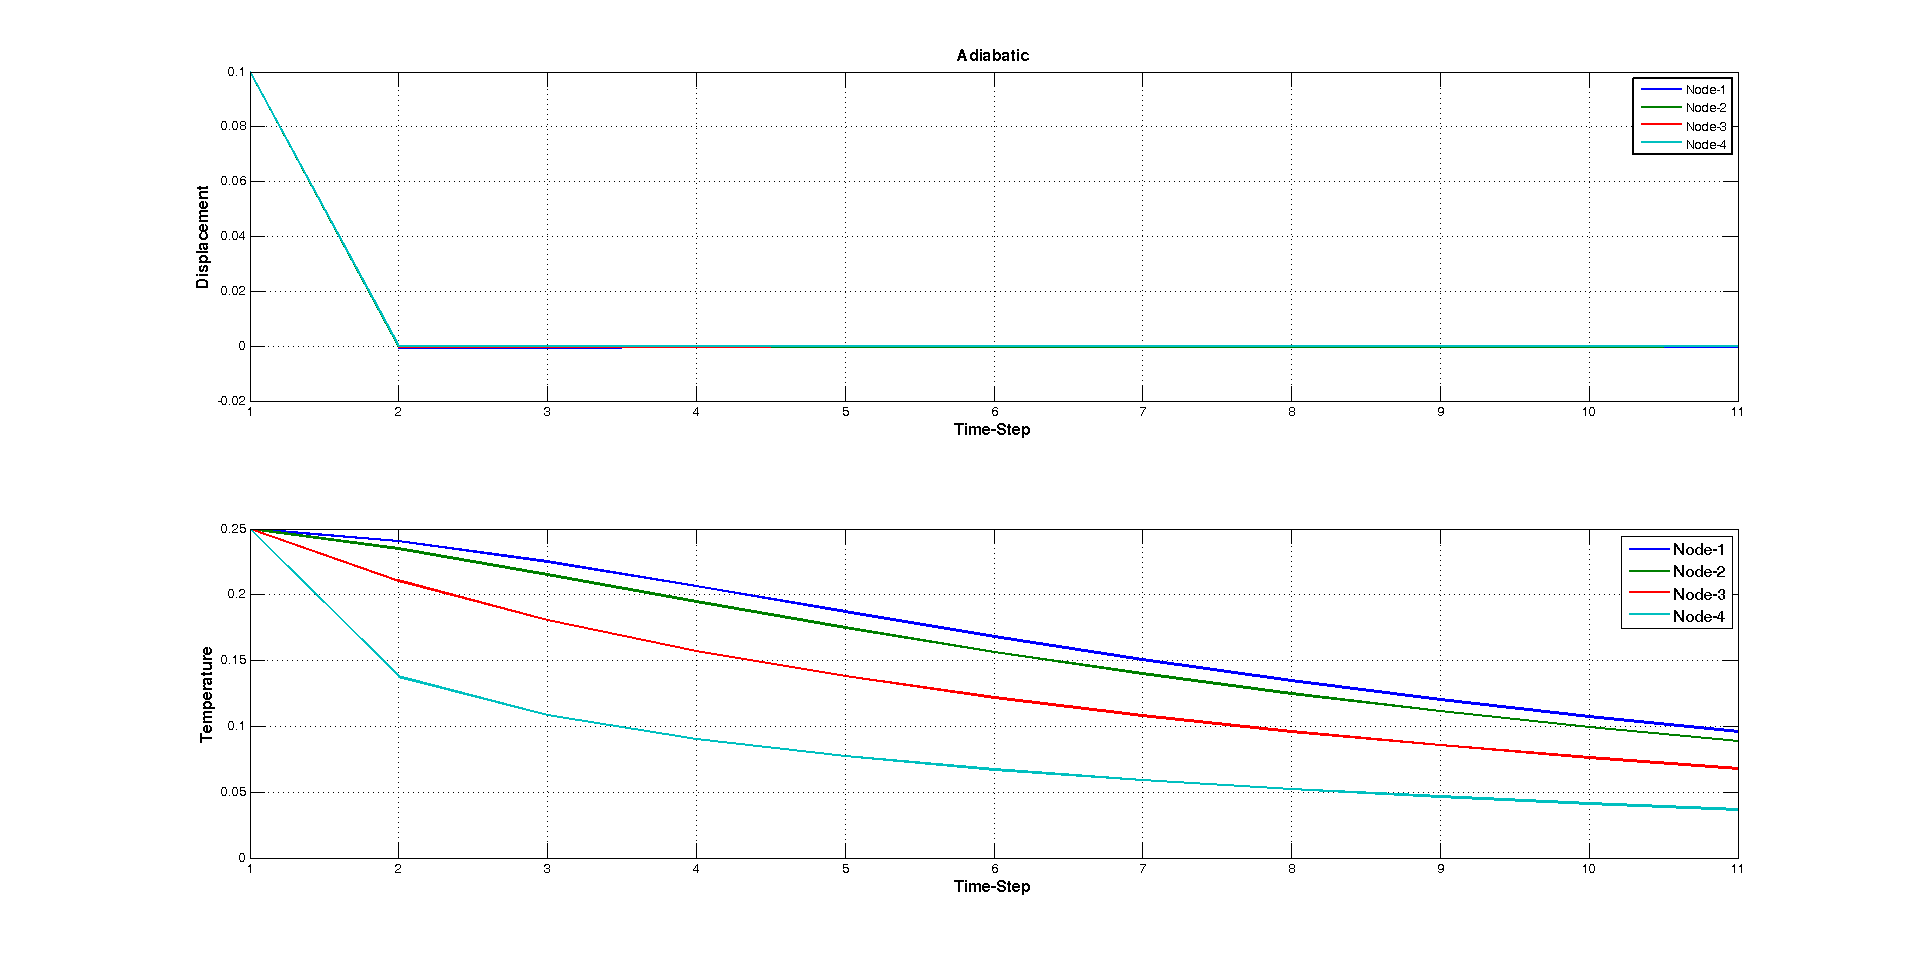
\includegraphics[width=7in,height=5in]{P2ad}
\end{center}\hrule
\subsection*{Comments: }
\begin{itemize}
\item The solution (both displacement and temperature) decay at similar rates for both linear and quadratic shape functions. 
\item There is a very slight difference in the temperature decay for node 3 (It decays slightly faster in case of linear shape functions). 
\item The rate of decay of temperature is the fastest for Node-4 and slowest for node 1 as node 4 is closest to the Dirichilet Boundary and Node 1 is the farthest. The plot for the Quadratic Shape functions is attached below. 
\end{itemize}
\begin{center}
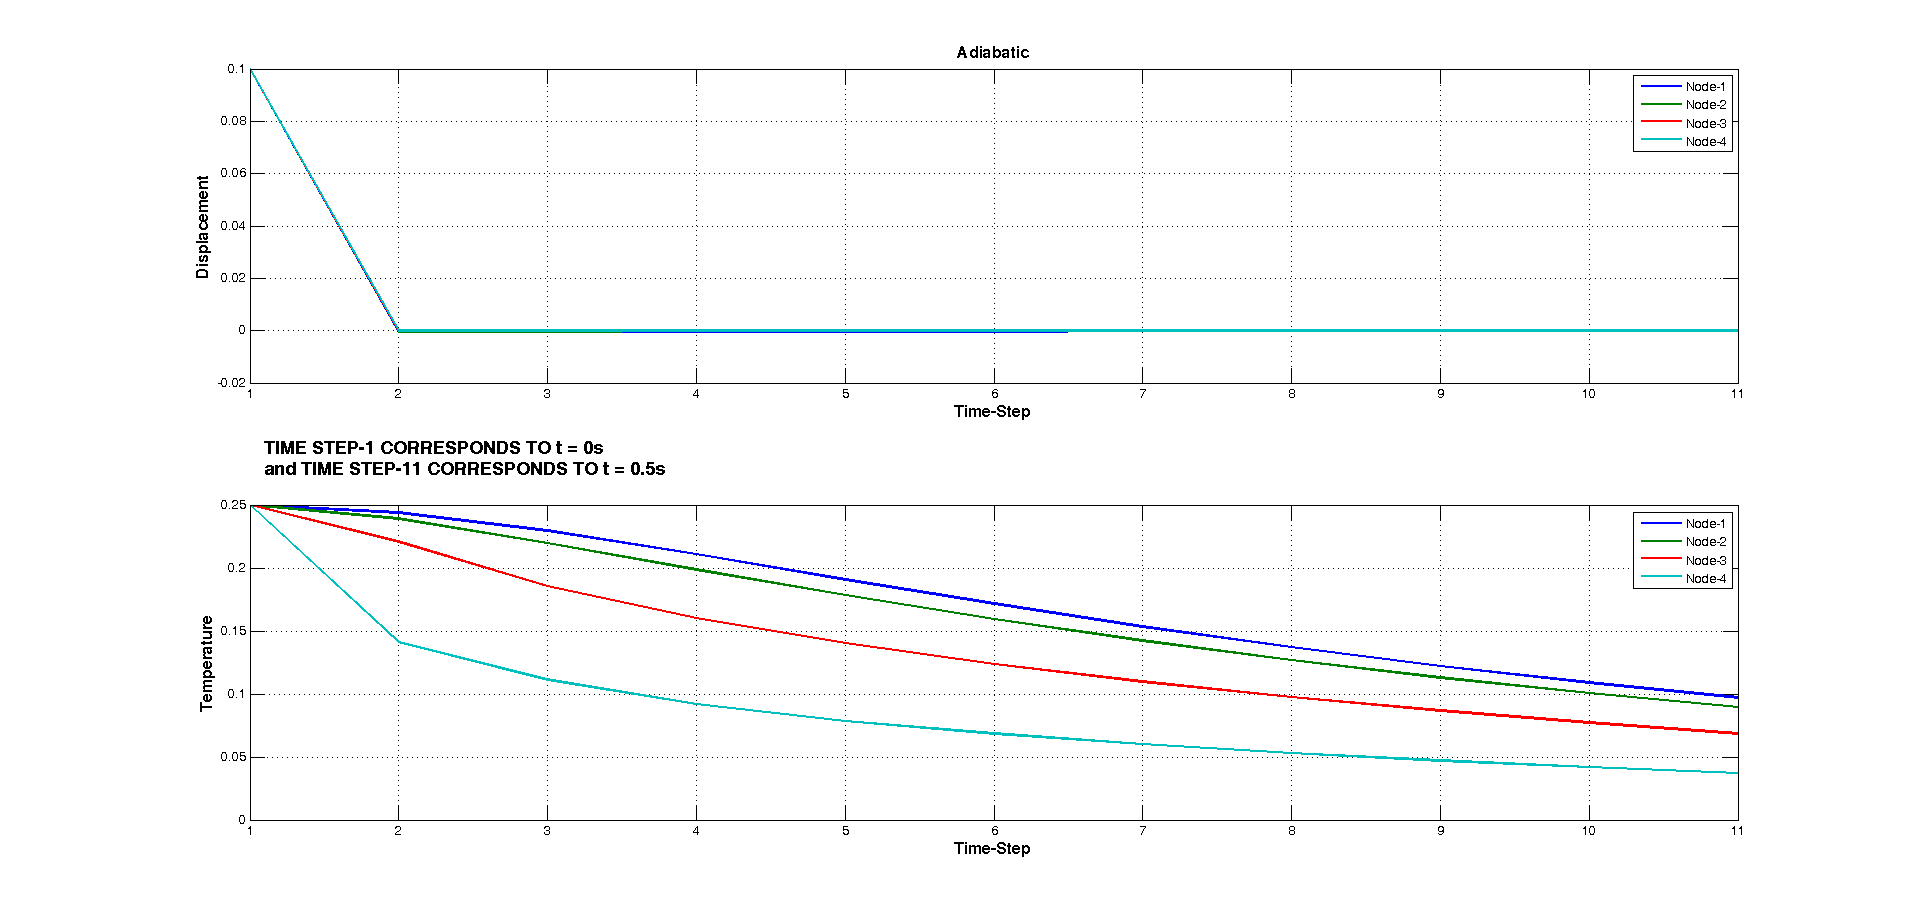
\includegraphics[width=7in,height=5in]{P3}
\end{center}\hrule
\begin{center}
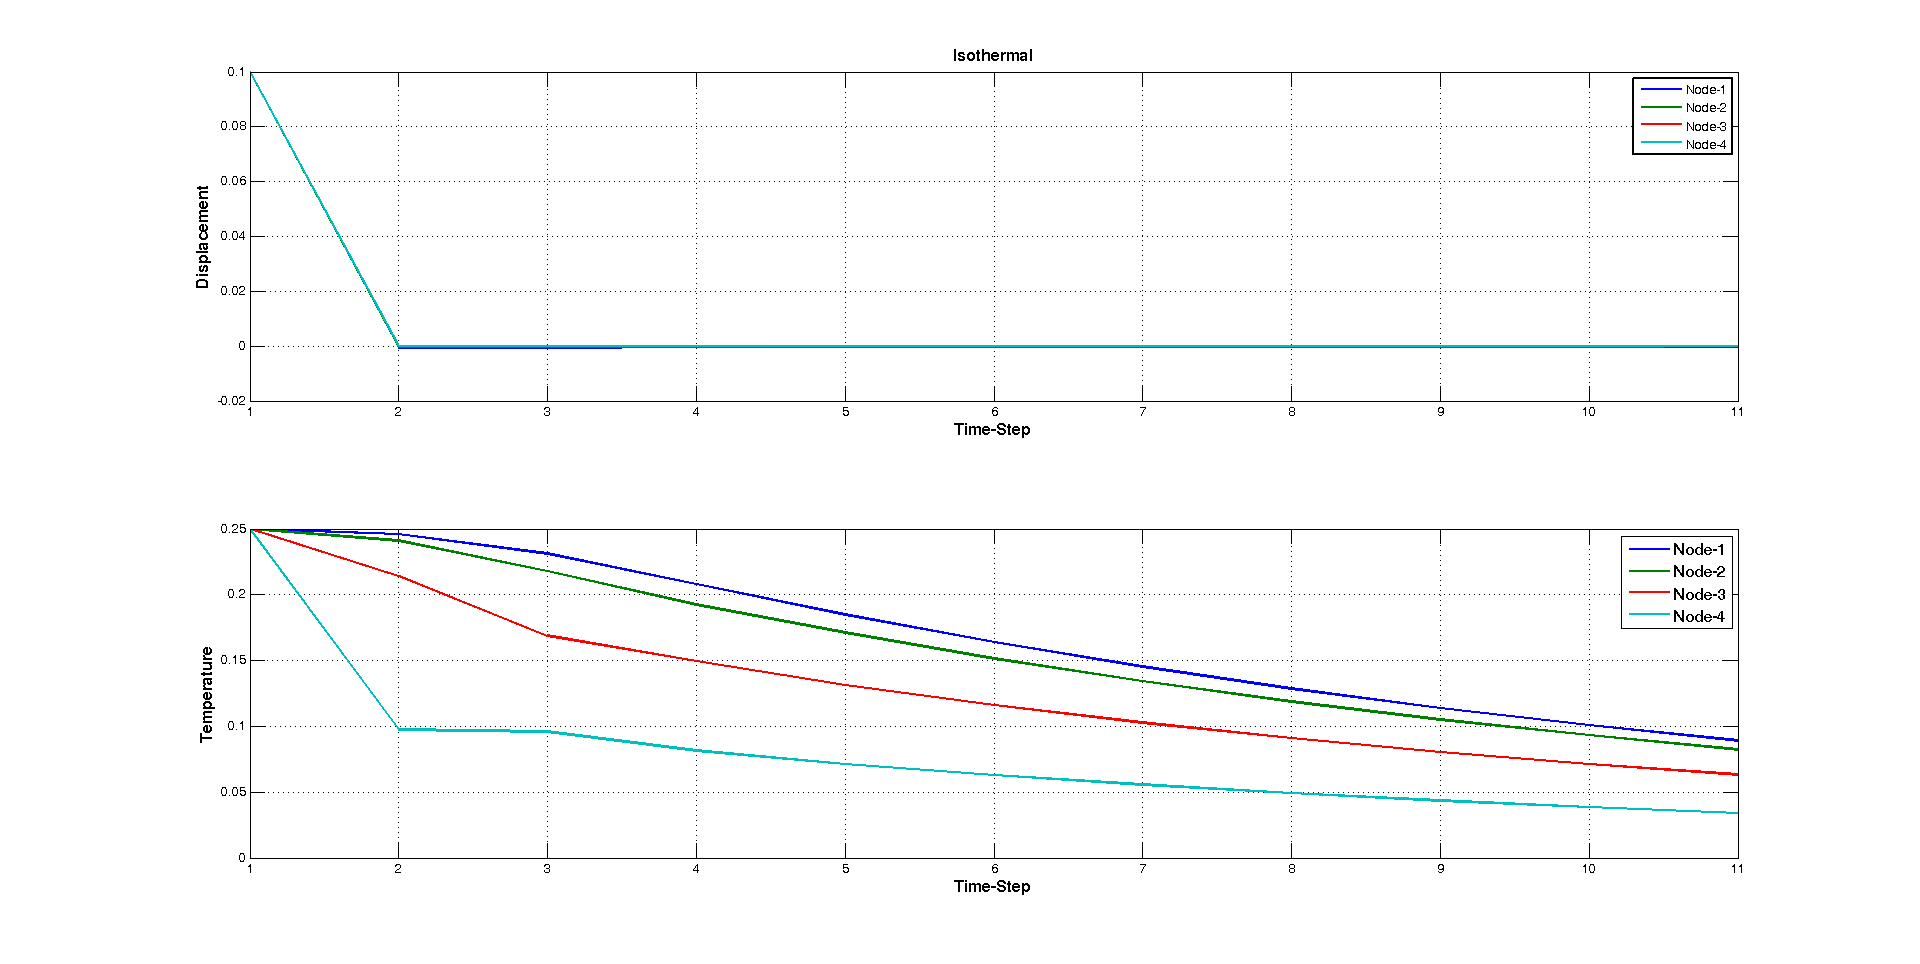
\includegraphics[width=7in,height=4.5in]{P2is}
\end{center}\hrule
\section*{Remarks (Bonus): }
For problem 1 and problem 2: 
\begin{itemize}
\item Both the Isothermal and adiabatic splits result in the convergence to the actual equilibrium (zero) solution. 
\item The temperature decay in case of Node-4 (closest to the Dirichilet) boundary is the fastest (as expected) among all the nodes. However as we can see that the corresponding plot in case of Isothermal has a flattening region (which is more profound in case of the larger time step, where it rises instead of decaying) around $t\approx2$. 
\item This can be attributed to the fact that the Isothermal split is only conditionally stable whereas the Adiabatic split is unconditionally stable. Therefore changing the value of $\Delta t$ has no effect on the Adiabatic split whereas it has on the Isothermal Split. (See Attached plot below)
\item It can be verified that the Adiabatic split remains stable for higher time steps, whereas Isothermal does not. 
\end{itemize}
\begin{center}
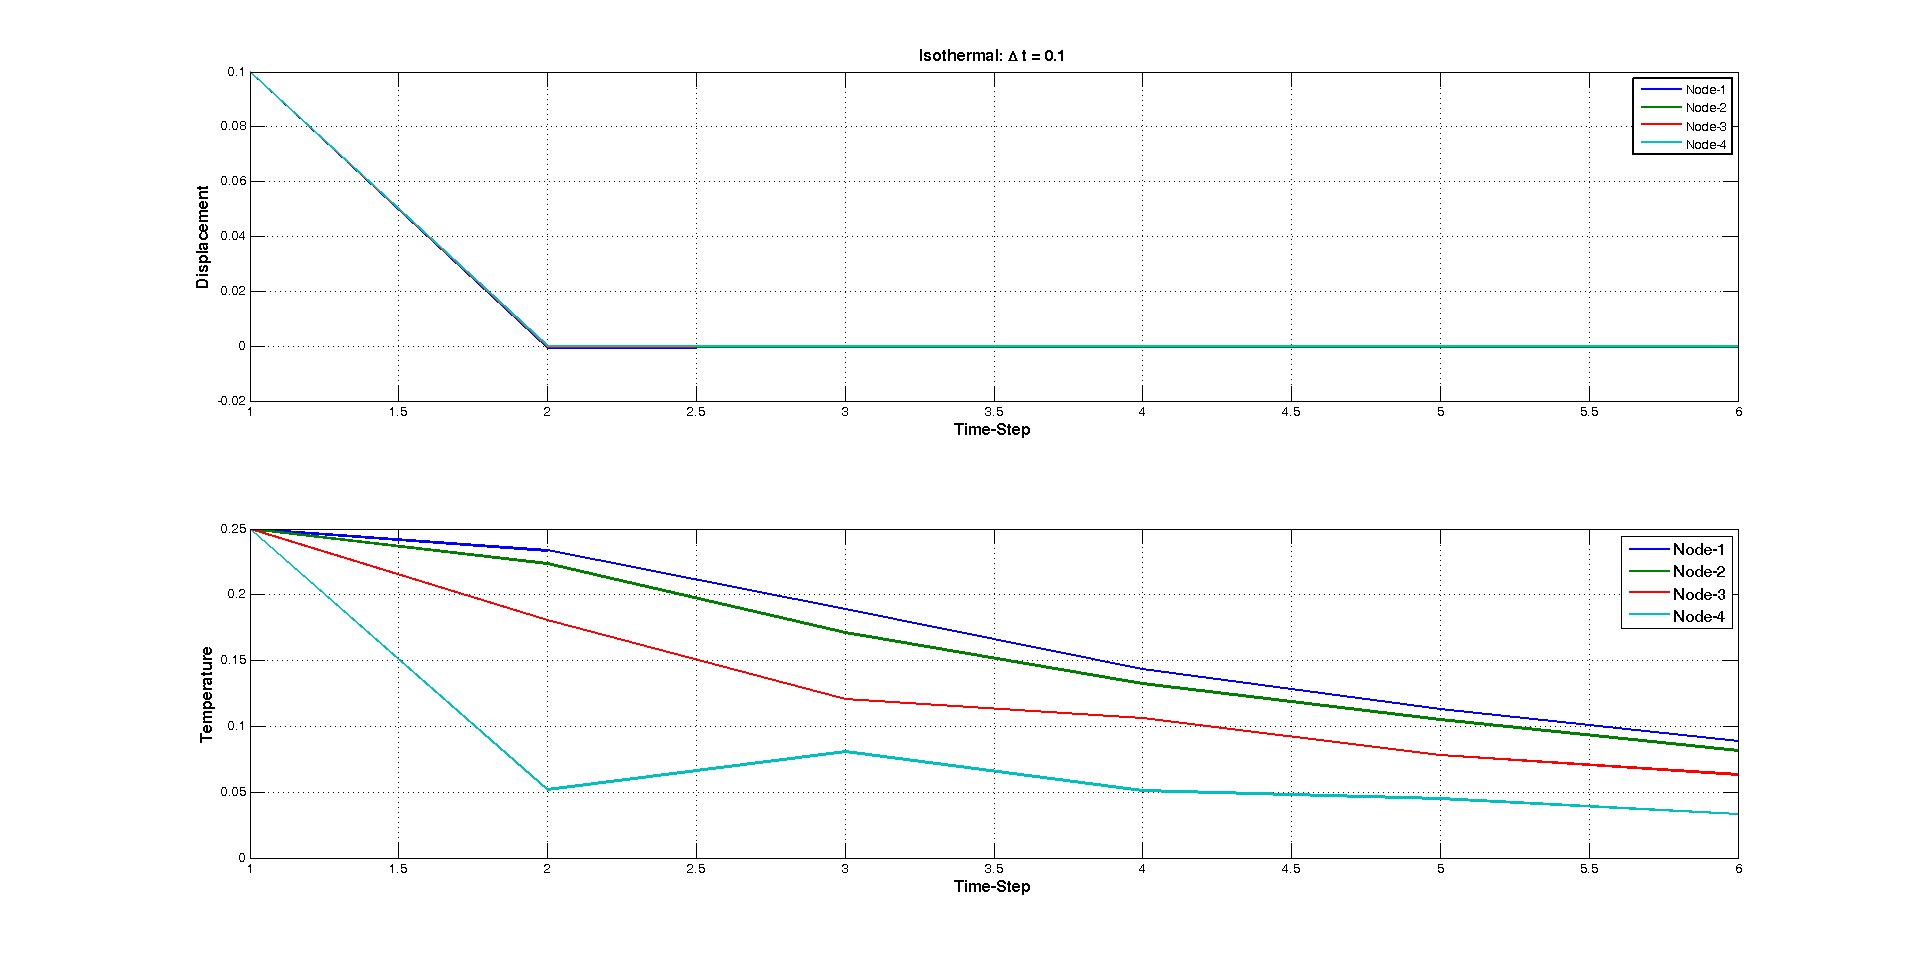
\includegraphics[width=7in,height=4.5in]{P2isdelt01}
\end{center}\hrule\hrule\hrule
\end{document}